\subsection{DLA by SAE Feature}
\label{sec:feature-resolved-component-decomposition}

We next ask where supporting readout features are written in the realized
residual stream.

\paragraph{Component-level readout terms.}
Because SRP is readout-linear, its feature terms compose with residual-stream
direct logit attribution (DLA)
\citep{elhage2021framework,wang2022ioi,nguyen2024logitprisms}. If
\(h\approx\sum_c h_c\), an SAE feature term for target \(q\) splits into
\[
    M_{c,i}(q)=\beta_i(q)\,h_c^\top d_i .
\]
For \(q=w_A-w_B\), \(\beta_i(q)=z_{A,i}-z_{B,i}\); for
\(q=w_A-\bar{w}_{\mathcal{V}}\),
\(\beta_i(q)=z_{A,i}-\bar{z}_{\mathcal{V},i}\). This yields additive
component-by-feature attribution from one forward pass. The same terms can serve
as inputs to later causal interventions \citep{geiger2023causalabstraction} that
test component or feature necessity.

\begin{figure}[!b]
    \centering
    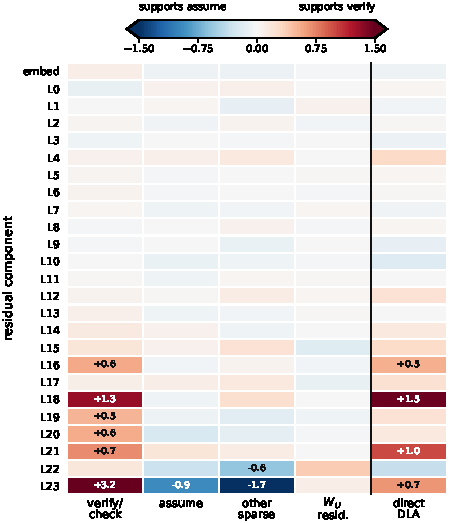
\includegraphics[width=0.86\columnwidth]{figures/proto_token_lens/qwen2b_32x_prism_dla_verify_assume/qwen2b_32x_prism_dla_semantic_table.pdf}
    \caption{\textbf{Feature-resolved component attribution for a
    \texttt{verify}-\texttt{assume} margin.}
    Rows are residual components; columns group feature families, unembedding
    residual, and ordinary DLA. Red supports \texttt{verify}; blue supports
    \texttt{assume}.}
    \label{fig:qwen-prism-dla-verify-assume-main}
\end{figure}

\Cref{fig:qwen-prism-dla-verify-assume-main} applies this decomposition to a
Qwen3.5-2B
\texttt{verify}-minus-\texttt{assume} target. The exact margin is \(+4.31\), the
residual-stream DLA sum is \(+4.36\), and the sparse feature sum is \(+4.28\)
(\(\rho=0.009\)), separating verification/checking support from
assumption-family opposition. A row-centered \texttt{verify} companion appears in
Appendix~\ref{app:feature-resolved-dla}.

\subsection{Readout Feature Edits Move Held-Out Lexical Scores}
\label{sec:readout-feature-edits}

Finally, we test whether SRP directions selected by a local account act as
narrow readout-side controls.

\paragraph{Constrained readout edit.}
We edit logits along ten Qwen3.5-2B decoder directions selected from five
discovery terms, then measure candidate-constrained lexical logit differences on
discovery and disjoint held-out tokens.

\begin{table}[H]
\caption{\textbf{Qwen3.5-2B readout edit.}
All methods use intervention scale \(16\). \(\Delta p_{\mathrm{bad}}\) is
reported as a positive reduction in probability assigned to the profane-token
side of held-out candidate pairs; median KL is next-token distribution shift.}
\label{tab:main-readout-edit}
\centering
\scriptsize
\setlength{\tabcolsep}{2.6pt}
\renewcommand{\arraystretch}{1.06}
\begin{tabular}{@{}lrrrr@{}}
\toprule
Method & \makecell{Disc.\\flip} & \makecell{Held-out\\flip} &
\makecell{Held-out\\\(\Delta p_{\mathrm{bad}}\)} &
\makecell{Median\\KL} \\
\midrule
SRP features (10) & \(0.450\) & \(0.359\) & \(0.398\) & \(0.679\) \\
Discovery token bias & \(0.450\) & \(0.000\) & \(0.000\) & \(0.001\) \\
Oracle token bias & \(0.450\) & \(0.359\) & \(0.404\) & \(0.004\) \\
Random features & \(0.013\) & \(0.156\) & \(0.078\) & \(1.363\) \\
No intervention & \(0.000\) & \(0.000\) & \(0.000\) & \(0.000\) \\
\bottomrule
\end{tabular}
\end{table}

\Cref{tab:main-readout-edit} shows that SRP features selected from discovery
tokens move held-out lexical logit differences (flip rate \(0.359\)), matching
an oracle token-bias edit while a discovery-token-only bias has no held-out
effect. R1-Distill-Qwen-7B shows the same pattern
(Appendix~\ref{app:lexical-control-stress-test}). This establishes readout-score
control for the specified lexical target.

\FloatBarrier
